\documentclass[logos,chaptertoc]{bordeaux-thesis}

%########################################################################
% Extensions
%########################################################################

%Text encoding and fonts
\usepackage[utf8]{inputenc}
\usepackage[T1]{fontenc}
\usepackage{autiwa-macros}
%\usepackage{graphicx}

% for the french text adaptation (babel is already in the class)
\FrenchFootnotes % pour les notes de bas de page
\AddThinSpaceBeforeFootnotes % pour les puristes (donc tout le monde!) qui veulent une espace fine entre le mot et l'appel de note


\renewcommand\theequation{\thechapter.\arabic{equation}}
\makeatletter
\@addtoreset{equation}{chapter}
\makeatother

\usepackage{natbib}%améliore la bibliographie, surtout pour citer les publications scientifiques.
\usepackage{frbib}%pour mettre la bibliographie en français
\usepackage{aas_macros}% contient les macros pour la définition des noms de journaux des publications scientifiques utilses pour les enterées bibtex de ADS.
\usepackage[nottoc]{tocbibind}%pour que la bibliographie  et l'index apparaissent dans la table des matières. l'option permet de ne pas afficher la table des matières. (notlof, notlot pour table des figures et ou des tableaux)

\usepackage{xspace}%Permet à babel d'utiliser la macro xspace  partout où c'est nécessaire. (Voir la doc de babel pour de plus amples explications.)

%########################################################################
% Title page
%########################################################################

%Thesis author
\author{Christophe \textsc{Cossou}}

%Title for main language (french)
\title{Migration et accrétion d'embryons planétaires dans un disque radiatif}
%Titles for other languages
\title[english]{My English thesis title}


%Keywords for main language (french)
\keywords{Blabla, blabla, blabla, blabla, blabla, blabla, blabla}
%Keywords for other languages languages
\keywords[english]{Blabla, blabla, blabla, blabla, blabla, blabla, blabla}

%Order number of the thesis
\ordernumber{1234}

%Date of defense
\date{xx Xxxxxxxxx xxxx}
\submityear{2013}

%You define the commission member list using \addcommissionmember (mandatory) with an optional role (eg: president, supervisor, etc...)
\addcommissionmember{Aaaaa}{Bbbbbbbb}{Astronome, Université Paris VI, LESIA}{Président du Jury}
\addcommissionmember{Ccccccccc}{Dddddddddd}{Directeur de recherche, Université Bordeaux 1, LAB}{Directeur de thèse}
\addcommissionmember{Eee}{Fffff}{Maître de conférence, Université Bordeaux 1, LAB}{Examinateur}
\addcommissionmember{Ggggggggg}{Hhhhhhh}{Professeur, Aix-Marseille, Université OAMP}{Examinateur}
\addcommissionmember{Iiii}{Jjjjjjjjjjjj}{Professeur, Aix-Marseille, Université OAMP}{Examinateur}
\addcommissionmember{Kkkkkkkkkkkk}{Llllll}{Professeur, Aix-Marseille, Université OAMP}{Examinateur}

%If some referees are not part of the commission, you can add them in a separate list with \addreferee (optional)
\addreferee{Mmmmmmmm}{Nnnnnnnn}{Professeur, Aix-Marseille, Université OAMP}
\addreferee{Oooooooooo}{Pppppppp}{Maître de conférence, Université Bordeaux 1, LAB}
%\addreferee{toto}{Pppppppp}{Maître de conférence, Université Bordeaux 1, LAB}

\newcommand{\dummytext}{
Lorem ipsum dolor sit amet, consectetuer adipiscing elit. Phasellus blandit massa non tellus. Pellentesque blandit. Etiam sapien. Quisque sed massa ac tortor accumsan bibendum. Donec et orci quis mi sollicitudin consectetuer. Donec malesuada. Pellentesque bibendum pellentesque elit. Morbi et diam ac wisi auctor fringilla. Cras nec arcu sed velit dapibus blandit. Maecenas mollis aliquet quam. In eget sem nec orci fringilla sagittis. Suspendisse cursus placerat massa. Pellentesque non metus. Morbi congue tellus eget tellus. Suspendisse justo. Suspendisse potenti. Praesent interdum lorem in velit. Nullam sit amet nisl eget wisi consectetuer consequat. Mauris vel felis. Nulla sed neque.

Nulla facilisi. Maecenas accumsan gravida wisi. Maecenas sodales gravida neque. Mauris in est a ante molestie gravida. In id neque. Ut augue. Duis fringilla ullamcorper risus. Nullam at lorem. Quisque consequat turpis ac libero. Ut auctor ante commodo magna. Donec in magna. Integer sodales. Donec ac nibh eu felis suscipit elementum.

Fusce convallis dolor sit amet dolor. Nulla sit amet pede. Maecenas et ante vitae risus tempus facilisis. Nullam ut tellus et lacus sollicitudin condimentum. Maecenas vitae lorem. Quisque nec leo varius est euismod posuere. Integer ac diam in enim pellentesque pulvinar. Etiam sodales tristique eros. Curabitur non magna. Suspendisse blandit metus vitae purus. Phasellus nec sem vitae arcu consequat auctor. Donec nec dui. Donec sit amet lorem vel erat tristique laoreet. Duis ac felis tincidunt arcu consequat faucibus. Vestibulum ultrices porttitor purus. In semper consequat dolor. Nunc porta. Vestibulum nisl ipsum, rhoncus quis, adipiscing sed, sollicitudin ut, quam.
}


%########################################################################
% Document start
%########################################################################

\begin{document}

%Print title NOW
\maketitle%

%Disable page numbering
\pagestyle{empty}

%########################################################################
% Multilingual abstracts
%########################################################################

%French abstract:
\begin{abstract}
\dummytext
\end{abstract}

%Horizontal rule
\noindent\hspace*{0.35\textwidth}\hrulefill\hspace*{0.35\textwidth}\\[-\bigskipamount]

%English abstract:
\begin{abstract}[english]
\dummytext
\end{abstract}

%########################################################################
% Acknowledgments
%########################################################################

\pagebreak\strut\newpage

\chapter*{Remerciements}
%Put the text vertically centered
\vfill
\dummytext
\vfill

\newpage

%########################################################################
% Contents
%########################################################################

\strut\newpage

\tableofcontents

\newpage

%########################################################################
% Introduction
%########################################################################

%Enable page numbering
\pagestyle{fancy}

\chapter*{Introduction}
\addstarredchapter{Introduction}% To be used instead of addcontentsline in order to have the good minitoc. If not, the starred chapter create a shift in the minitocs.
%%\addcontentsline{toc}{chapter}{Introduction}

%TODO parler de formation planétaire (en citant des papiers, sans rentrer dans les détails. notamment pollack, alibert)

%TODO une des grandes questions c'est  : comment on forme des noyaux de jupiter et Kepler 11?



\chapter{Physique des disques}
\section{Les disques protoplanétaire}
%TODO voir thèse mordasini, et les articles de mordasini, alibert, ida et lin, histoire de voir ce qu'ils font)
\subsection{Formation et évolution}
%TODO 
\subsection{La viscosité du disque} \index{viscosité}% (Franck et al. 1992)
Quand on parle de viscosité $\nu$ dans un disque, ce n'est pas la viscosité moléculaire classique. On suppose généralement une viscosité due aux turbulences qui est beaucoup plus importante que la viscosité moléculaire, mais qui peut être traitée par les mêmes équations. 

La première hypothèse est de considérer une viscosité constante. Faute de mieux, c'est ce qui semble être le plus évident. On peut, si on veut affiner, utiliser une théorie dite des \gras{disque-alpha}

\subsubsection{Les disques alpha}
On peut introduire un paramètre adimensionné $\alpha$ \citep{shakura1989black}. Dans ce formalisme, plusieurs hypothèses sont faites : 
\begin{itemize}
\item On considère que les turbulences sont sub-soniques.
\item L'échelle des tourbillons des turbulences est plus petite que l'échelle de hauteur du disque
\end{itemize}

En conséquence, on peut définir la viscosité $\nu$ associée aux turbulences comme étant 
\begin{align}
\nu &= \alpha c_s H
\end{align}
où $c_s$ est la vitesse du son et $H$ l'échelle de hauteur du disque. $\alpha$ (avec $\alpha < 1$) est alors un paramètre adimensionné qui permet de définir plus ou moins l'intensité des turbulences, et donc la viscosité qui leur est associée. Une valeur typique d'$\alpha$ se situe entre $10^{-2}$ et $10^{-4}$.

Même si cette prescription simplifie un peu le problème, il semble probable qu'$\alpha$ ne soit pas constant, et dépende de la position dans le disque. On déplace alors le problème, vu que se pose la question des variations d'$\alpha$ dans le disque, notamment la dépendance radiale de ce dernier.

\bigskip

Le mécanisme qui a le plus de chance d'être à l'origine de la viscosité alpha est l'\gras{Instabilité Magnéto-Rotationnelle} (MRI). 

\subsection{Ionisation et dead-zones}\index{ionisation}\index{dead zone}
Pour qu'une instabilité magnéto rotationnelle ait lieu, c'est à dire qu'il y ait un couplage entre le champ magnétique et les mouvements du disque, il faut qu'une partie au moins du disque soit ionisé. Dans ces régions ionisé, on pourra alors avoir transport du moment angulaire via la viscosité due au champ magnétique (et turbulences engendrées). 

Or, comment ioniser? Que ce soit le rayonnement X de l'étoile centrale, des rayons cosmiques ou l'ionisation thermique, il n'est pas si évident que ça de se représenter l'ionisation totale du disque de gaz. Il est donc probable que certaines zones du disques ne soient pas ionisés, et donc que le transport du moment angulaire s'y fasse peu ou pas du tout. Ces zones, appelées \index{dead zone}, sont donc des zones sans viscosité magnétique. %TODO compléter la partie dead zone

\begin{figure}[htb]
\centering
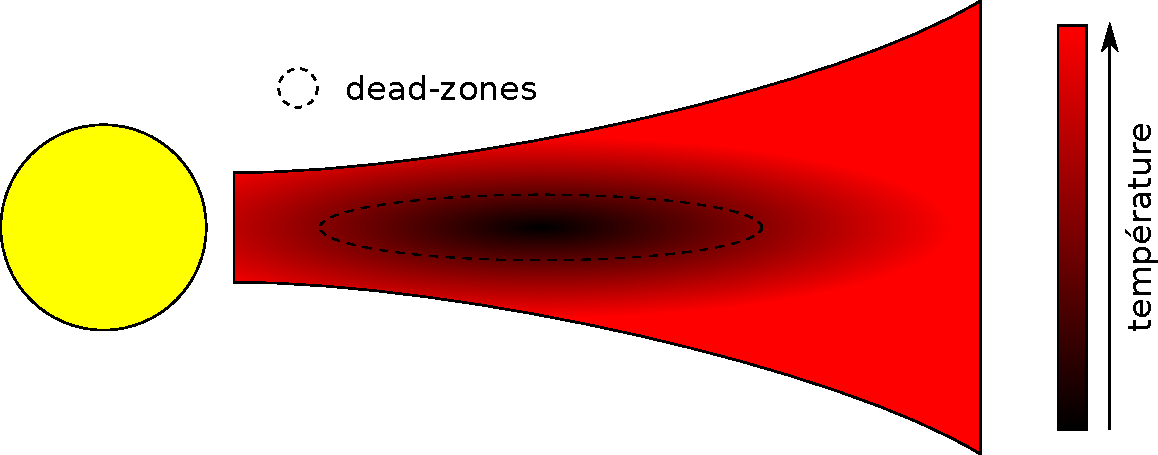
\includegraphics[width=0.7\linewidth]{figure/dead_zones.pdf}
\caption{Représentation d'un disque à couches (layered disk). L'ionisation d'une zone est déterminé par sa température. Ainsi, les zones internes à température plus faible ne sont pas ionisés et n'ont donc pas de viscosité dûes aux turbulences magnétique (MRI). Les régions externes ne sont pas des zones mortes parce qu'elles peuvent être sujettes à des ionisations non thermiques en raison de leur densité plus faible. À distance intermédiaire, le disque est trop froid pour de l'ionisation thermique, et trop dense pour de l'ionisation non thermique.}\label{fig:dead_zones}
\end{figure}


%TODO j'en suis à la page 158 du .pdf ``accretion processes in star formation''

\subsection{Profil de densité}
%TODO 
\subsection{Profil de température}
Du point de vue de la température, il y a principalement deux types de disques : 
\begin{itemize}
\item les \gras[disque actif]{disques actifs} : la source de température est le disque lui même, qui par frottements visqueux (on appelle ça le \gras{chauffage visqueux}) va émettre de la chaleur, et donc chauffer le disque ;
\item les \gras[disque passif]{disques passifs} : la source de chaleur/température est l'étoile centrale qui éclaire le disque. 
\end{itemize}

Un disque peut à la fois être actif et passif, mais généralement on essaie d'approximer, de considérer que l'un est négligeable devant l'autre. De plus, un disque aura des zones actives et des zones passives, c'est à dire que certaines zones seront principalement chauffées par la viscosité alors que d'autres le seront par l'\gras{irradiation de l'étoile}.
%TODO parler de la température du disque (et les phénomènes principaux qui ont un effet sur la température, chauffage visqueux, irradiation de l'étoile, irradiation externe. Parler dans cette partie de l'opacité, des transitions et à quoi c'est dû, des modèles had oc pour l'opacité et des incertitudes qui en découlent

\subsection{Les bords du disque}
%TODO parler des bords du disque et de tous les problèmes que ça pose

\section{Interaction disque-planète}
\subsection{Migration planétaire}
%TODO 
\subsubsection{Type I}\index{migration!type I}
Ce type de migration ne concerne que les planètes de faible masse (de l'ordre de $10M_{\oplus}$)pour lesquelles l'interaction de marée entre la planète et le disque a une réponse linéaire (Le profil de densité surfacique reste quasiment le même). Ces planètes, qui ne creusent pas de sillon (gap) dans le disque de gaz, vont migrer vers l'intérieur.

\begin{remarque}
Pour plus de détails, se référer au chapitre 9, page 188--191 de \cite{barnes2010formation} ou \cite{ward1997protoplanet} pour l'article original.
\end{remarque}

La présence d'une planète dans un disque de gaz entraine la création d'ondes de densités aux \gras[résonnance!de Lindblad]{résonances de Lindblad} \citep{goldreich1979excitation}. Le couplage gravitationnel entre les ondes de densité et la planète qui les crées abouti à un \gras{couple} qui agit sur la planète.

Lors de la création d'ondes de densité par une planète dans un disque, il se forme un déséquilibre naturel entre les couples agissant sur les disques internes et externes. La position des résonances de Lindblad externes tend à être plus proche de la planète que ne l'est celle des résonances internes.


%TODO 
\subsubsection{Type II}\index{migration!type II}
Quand une planète dans un disque devient suffisamment massive, la réponse du disque n'est plus linéaire, et des ondes de densité induites par la planète forment des chocs non loin de là où elles sont émises. La répulsion entre le disque et la planète devient si forte qu'une cavité annulaire se forme autour de l'orbite de la planète, creusant le disque de gaz.

Une fois que la cavité est formée, la planète est dite en migration de \emph{type II} : son orbite agit alors essentiellement comme une barrière entre les deux parties du disque de gaz, \emph{interne} et \emph{externe}. Du gaz peut parfois sauter le gap, ou être accrêté par la planète mais cette dernière voit son mouvement régit par le disque de gaz, se retrouvant entraînée par la migration de celui-ci.

Compte tenu que la planète a une masse de l'ordre de\footnote{Quand la masse de la planète devient supérieure à la masse du disque local, l'inertie de celle-ci devient importante afin de déterminer son taux de migration} la masse du disque local (avec lequel elle interagit), la migration se passe sur des temps de l'ordre du \gras{temps visqueux} du disque.

\begin{remarque}
Pour plus de détails, se référer au chapitre 9, page 191--192 de \cite{barnes2010formation} ou \cite{lin1986tidal} pour des détails sur les planètes capables de former un sillon dans le disque de gaz.
\end{remarque}
%TODO 
\subsubsection{Type III}\index{migration!type III}

%TODO faire ya page 192 du bouquin de barnes un truc sur \c ca, même si c'est pas explicite dans le titre.

\begin{remarque}
Pour plus de détails, se référer au chapitre 9, page 192--193 de \cite{barnes2010formation} ou \cite{masset2003runaway}.
\end{remarque}
%TODO 

\subsection{L'amortissement de l'excentricité}%circularisation
%TODO parler des autres phénomènes importants dans le disque, comme l'amortissement de l'excentricité

\subsection{L'amortissement de l'inclinaison}%coplanarisation
%TODO parler de l'amortissement de l'inclinaison, 

\subsection{L'accrétion du gaz}\label{sec:accretion_coeur}
Dans le modèle d'\gras[modèle!accrétion de c\oe ur]{accrétion de c\oe ur}, les planètes géantes sont d'abord des c\oe urs rocheux qui grossissent jusqu'à atteindre une masse critique de l'ordre de $15 M_{\oplus}$. Une fois cette masse atteinte, le c\oe ur commence à accréter rapidement du gaz jusqu'à former une géante gazeuse.

Ceci implique que la formation des planètes géantes doive se passer avant que le disque de gaz ne se dissipe (ce qui intervient au bout de $10^7$ ans environ).

Les noyaux de ces planètes sont supposés se former au delà de la ligne des glaces (limite radiale virtuelle au delà de laquelle on peut trouver de l'eau sous forme solide ; autour de $4\unit{ua}$). En effet, au delà de cette limite, la quantité de matière solide augmente, et donc le taux d'accrétion augmente aussi.

\begin{attention}
La formation des embryons de planètes géantes n'est toujours pas clair. On ne sait pas vraiment s'il y a une zone privilégiée ou non, la limite virtuelle de la ligne des glaces pourrait ne pas être valable, la glace ne rajoutant qu'environ 50\% de masse en plus.\index{ligne des glaces}\index{snowline|see{ligne des glaces}}

À noter qu'il n'y a pas de pression et donc pas de liquide dans l'espace, juste du gaz ou du solide.
\end{attention}

\bigskip

Pour une simulation donnée, si on augmente le taux d'accrétion de la planète, celle-ci sera plus massive, et aura donc une inertie plus grande. Elle mettra donc plus de temps à migrer\index{migration} par migration Type II car son inertie s'y opposera. D'un autre coté, si la planète n'a pas encore créé de gap, la migration de Type I est plus rapide à mesure que la masse augmente. 

%TODO parler de l'accrétion, et du fait que ça va créer des planètes géantes notamment

\subsection{Récapitulatif des interactions dans le code N-corps}
%TODO parler du fait que je ne prend pas en compte l'accrétion de gaz, les gaps, 

\chapter{Le Code N-Corps}
Afin d'étudier la formation planétaire et les interactions avec le disque de gaz, j'ai utilisé un code de simulation N-corps, qui permet de regarder l'évolution d'un nombre arbitraire de corps orbitant autour d'un astre central. 

Ce choix est apparu naturellement. Au début de ma thèse j'ai fait quelques simulations hydrodynamiques avec le code Genesis développé par Arnaud Pierens. J'ai rapidement constaté que ce genre de simulations, bien que modélisant de manière poussée le disque, ne permettait pas d'étudier de manière approfondie la dynamique planétaire. Le temps de calcul nécessaire pour une simulation limite en effet grandement le nombre de corps ainsi que la durée d'intégration. J'ai donc souhaité me tourner vers un code N-corps, afin de privilégier la dynamique planétaire, et de modifier ce programme afin d'y inclure les effets d'un disque de gas sur la dynamique planétaire. 

J'ai ainsi gagné en temps de calcul, et j'ai ouvert un vaste champ d'investigation sur les paramètres du disques, le nombre de corps en interaction, me permettant de faire des systèmes planétaires très divers, parfois avoir plusieurs centaines d'embryons pour plusieurs millions d'années, chose impossible dans les simulations hydrodynamiques du début de ma thèse où 20 corps pendant quelques dizaines de milliers d'années était un maximum. 

Ce choix a bien entendu introduit son lot d'incertitudes et d'approximations qui sont discutés dans la partie \refsec{sec:discussion}. La présente section a pour but de présenter le code N-corps que j'ai utilisé ainsi que les différents effets du disque que j'ai modélisé. J'ai avant tout souhaité présenter les parties qui ont des conséquences sur la physique du disque, que ce soit en terme de choix d'un modèle particulier, ou de limitations numériques qu'il est bien de garder à l'esprit quand on interprète les résultats.

\section{Présentation de mercury}
Le code N-corps choisi est le code \textbf{mercury} \citep{chambers1999hybrid}. Ce code offre la possibilité de choisir un algorithme parmi 5 différents (BS, BS2, RADAU, MVS et HYBRID), ayant des propriétés diverses. Dans le cadre de ma thèse, je n'ai utilisé que l'algorithme HYBRID, qui utilise l'algorithme MVS la plupart du temps, mais change pour l'algorithme BS2 lors de rencontres proches. Il est possible de déterminer à quel moment on considère qu'une rencontre est "proche" dans le fichier de paramètre de programme, j'ai laissé le paramètre par défaut. 

La raison de ce changement est assez simple. MVS est un algorithme symplectique, c'est à dire à pas de temps constant, dans lequel on défini un hamiltonien que l'on résout pour faire évoluer les orbites. La conservation de l'énergie est moins bonne que pour un algorithme à pas de temps adaptatif, mais le point très important est que cette conservation de l'énergie est bien meilleure au cours du temps. C'est à dire que là où les algorithmes tels que BS, BS2 et RADAU verront leur erreur sur l'énergie augmenter au cours du temps, les algorithmes symplectiques vont eux voir leur erreur rester plus ou moins constante au cours du temps. 

Dans le cadre de mes simulations, j'ai accordé une importance limitée aux variations d'énergie, étant donné que les couples que l'on rajoute pour simuler la présence du disque de gaz font que l'énergie n'est pas conservée pour une planète donnée. Cependant, il est important de bien résoudre les orbites et c'est ce point qui est le plus crucial ici. En effet, quelques tests ont permis de contraindre le pas de temps minimal qu'il est nécessaire d'avoir en fonction de la distance orbitale d'une planète. La contrainte de pas de temps dans mes simulations vient donc d'une distance minimale en dessous de laquelle les orbites ne sont pas correctement calculées. Cette limite, afin d'éviter tout problème, est choisie pour être en dessous du bords interne du disque de gaz que je défini.

%TODO Simulation lancées dans le dossier $sse/test_mercury, sur une même simulation mais avec différents algorithmes pour voir l'évolution de la conservation de l'énergie au cours du temps

%TODO parler de la précision de conservation de l'énergie
%TODO parler du pas de temps qui a une influence sur les orbites, et des tests effectués pour contraindre le pas de temps par rapport à l'orbite minimale accessible.

\section{Disque 1D}
Afin de calculer les effets d'un disque de gaz, une modélisation de ce dernier est nécessaire. Le but étant d'avoir une grande souplesse, le disque implémenté est bien entendu très simplifié. Toutes les quantités sont intégrées et invariantes selon la hauteur z et la position azimutale $\theta$ dans le disque, résultant en un modèle radial de toutes les quantités. 

Dans la mesure du possible, les quantités du disque ont été calculées de manière consistante. Je vais présenter dans la suite de manière chronologique comment sont calculées les grandeurs physiques du disque.
%TODO 
\subsection{Profil de densité de surface}
Le profil de densité de surface est défini au début de la simulation comme une loi de puissance de la forme :
\begin{align}
\Sigma(R) &= \Sigma_0 \times R^{-\alpha}
\end{align}
où $\Sigma_0$ est la densité de surface à $1\unit{AU}$ et $\alpha$ l'indice de la loi de puissance. 

Ce profil de densité de surface est défini pour une certaine étendue radiale. On défini donc un bord interne $R_\text{in}$ et un bord externe $R_\text{out}$. Le bord interne est généralement à $0,1\unit{AU}$ et le bord externe à $100\unit{AU}$. 

Afin de calculer les valeurs suivantes, ce disque est échantillonné et toutes les valeurs nécessaires sont ensuite calculées à chacun de ces points. 

\subsection{Table d'opacité}
%TODO 
\subsection{Profil de température}
%TODO 
\section{Migration type I}
%TODO 
%TODO paardekooper
\section{Amortissement de e et I}
%TODO 
\section{Effet de l'excentricité sur le couple de corotation}
%TODO du couple de corotation quand l'excentricité augmente, mais je sais pas encore où le placer, pas dans la partie intro je suppose

\chapter{Mécanismes individuels}
\section{Les Résonances de Moyen Mouvement (MMR)}
\subsection{Définition}\index{résonance!de Moyen Mouvement}\index{Mean Motion Resonance|see{résonance}}
Les \gras[resonance@résonance]{résonances de moyen mouvement} sont des configurations orbitales particulières de deux planètes dans lesquelles il existe un lien entre les périodes orbitales des planètes. Exemple, si deux planètes sont en résonance $3:2$, ça signifie que la planète interne effectuera 3 orbites pendant que la planète externe en effectuera 2.

Ces configurations particulières confèrent une stabilité accrue aux planètes. Plus la résonance est forte et plus il sera difficile pour les planètes d'en sortir.

\bigskip

On met généralement une résonance sous la forme $(p+q):p$ où $p$ et $q$ sont des entiers. Cette forme permet de mettre en évidence un des paramètres qui permet de rendre compte de la force de la résonance. En effet, plus $q$ est petit et plus la résonance est force. Ainsi, les résonances avec $q=1$ sont les plus fortes. On dit que $q$ est l'ordre de la résonance (plus l'ordre est petit et plus la résonance est forte).

\begin{attention}
Mais ce n'est pas le seul paramètre à prendre en compte pour évaluer la force d'une résonance et je suis bien incapable de tous les décrire.
\end{attention}

Pour une résonance $(p+q):p$ on définit un certain nombre d'angles $\theta_i$ dits \gras[angle de résonance]{angles de résonance} de la forme :
\begin{align}
\theta_{i+1} &=(p+q)\lambda_2 -p\lambda_1 - \left[i\varpi_{1} + (q-i)\varpi_2\right]
\end{align}
avec $i$ allant de $0$ à $q$ ; où $\lambda$ sont les longitudes moyennes, $\varpi$ les longitudes du péricentre et les indices $1$ et $2$ se réfèrent respectivement à la planète interne et externe. Pour une résonance $(p+q):p$ on a donc $q+1$ angles de résonance.

Les angles de résonances mesurent l'angle entre les deux planètes au point de conjonction. Si un seul de ces angles est en libration (oscillation autour d'une valeur moyenne) au lieu de circuler librement de $0$ à $2\pi$ alors on dit que les planètes sont en résonances. Le nombre d'angles en libration permettra aussi d'avoir une idée de la force de la résonance.

\begin{exemple}
Soit une résonance $7:2$, les angles de résonances sont :
\begin{align*}
\theta_1 &= 7 \lambda_2 -2\lambda_1 - 5 \varpi_1\\
\theta_2 &= 7 \lambda_2 -2\lambda_1 - \left( 4 \varpi_1 + 1\varpi_2 \right)\\
\theta_3 &= 7 \lambda_2 -2\lambda_1 - \left( 3 \varpi_1 + 2\varpi_2 \right)\\
\theta_4 &= 7 \lambda_2 -2\lambda_1 - \left( 2 \varpi_1 + 3\varpi_2 \right)\\
\theta_5 &= 7 \lambda_2 -2\lambda_1 - \left( 1 \varpi_1 + 4\varpi_2 \right)\\
\theta_6 &= 7 \lambda_2 -2\lambda_1 - 5 \varpi_2
\end{align*}
\end{exemple}

\begin{remarque}
Les \gras[kirkwood@Kirkwood!lacunes de]{lacunes de Kirkwood} font elles aussi intervenir des résonnances mais contrairement à ce qu'on pourrait penser, ces résonances avec Jupiter sont des zones déplétées en astéroïdes. La raison profonde n'est pas parfaitement connue mais il semblerait que ce soit dû au chaos. Je ne saurais pas expliquer exactement ce que ça veut dire par contre.

La résonance imposte une valeur de $a$, mais des échanges sont possibles entre les deux corps en résonance (je ne sais pas bien de quelles valeurs par contre), et il est possible que par ce biais l'eccentricité puisse augmenter, et ainsi dépléter la lacune de kirkwood en favorisant les collisions entre les objets en résonance et les autres qui sont dans la ceinture.
\end{remarque}
%TODO MMR : lire a thorough analysis of the dunamics involved the reader should consult (Murray & Dermott, 1999)
%TODO 
\subsection{Résonances et excentricité}
%TODO 
\subsection{Stabilité et ordre des résonances}
%TODO 

\section{Les Zones de Convergence}
%TODO 
\subsection{Existence et intérêt}
%TODO 
\subsection{Les différents types}
%TODO 
\subsection{Diagrammes de couple a-m}
%TODO parler des raisons pour lesquelles la zone de convergence dépend de la masse et de la distance parfois, avec les comparaisons des temps (dynamique, de U-turn and de diffusion)
\subsection{Résonances et Accrétions}
%TODO 

\chapter{Mécanismes de formation}
\section{Décalage de la Zone de Convergence}
%TODO 
\section{Formation des super terre chaude}
%TODO 
\section{Effets des paramètres du disque}
%TODO 
\subsection{Viscosité du disque}
%TODO 
\subsection{Profil de densité de surface}
%TODO 
\subsection{Profil de température}
%TODO 
\subsection{Masse du disque}
%TODO 
\subsection{Table d'opacité}
%TODO 

\chapter{Discussion et limite du modèle}\label{sec:discussion}
\section{Étude de sensibilité}
%TODO 
\subsection{Le choix de la table d'opacité et son implémentation}
%TODO le choix de la table, mais aussi le fait qu'on a besoin d'une densité volumique, ou qu'on a besoin de la masse moléculaire moyenne. 

\subsection{Modélisation de la viscosité}
%TODO 



\section{Approximations}
%TODO 
\subsection{Profil de densité du gaz en 2D}
%TODO 
\subsection{La modélisation des bords du disque}
%TODO 
\subsection{Pas d'effet indirect des ondes de densité sur les autres planètes}
%TODO 
\subsection{Auto-gravité}
%TODO 

\chapter*{Conclusion}
\addstarredchapter{Conclusion} % to be used in place of addcontentsline to avoid problems with minitoc
%%\addcontentsline{toc}{chapter}{Conclusion}

\dummytext

%TODO 

%\thispagestyle{empty}
%\strut\newpage

\bibliographystyle{plainnat}
\bibliography{these}%.bib

\end{document}
